\documentclass{beamer}

\usepackage[utf8]{inputenc}
\usepackage{graphicx}
\usetheme{Berkeley} 
\usecolortheme{default}
\setbeamertemplate{footline}[frame number]

%% Title frame info
\title{Licence Pro ADSILLH}
\subtitle{Projet Big Data}
%% \institute{ADSILLH}
\author{Pierre-Antoine Rouby\\Lunix}
\date{Année 2017/2018}
\logo{
\includegraphics[width=1.5cm]{../images/logo_univ.jpg}}

% ce code permet d'afficher le sommaire à chaque section,
% en mettant en valeur la section courante (utile ?)
% \AtBeginSection[]
% {
%   \begin{frame}
%     \frametitle{Sommaire}
%     \tableofcontents[currentsection]
%   \end{frame}
% }

\begin{document}
\frame{\titlepage}

\begin{frame}
  \frametitle{Sommaire}
  \tableofcontents
\end{frame}

\section{Présentation}
\begin{frame}
  \frametitle{Les besoins}

  Le but du projet et d'inventer une application permettant de se passer
  des agences immobilière tous en gardent le même niveaux de service
  et de fiabilité.
  \begin{columns}
    \column{0.6\textwidth}
    \begin{itemize}
    \item Calcule automatique de la valeur d'un bien
      \begin{itemize}
      \item Géolocalisation
      \item Plan
      \item États de l'appartement par photos
      \end{itemize}
    \end{itemize}
    \begin{itemize}
    \item Visite en ligne
      \begin{itemize}
      \item VR (Virtual Réality)
      \end{itemize}
    \end{itemize}
    \column{0.4\textwidth}
    
\includegraphics[scale=1]{../images/geo.jpg}
    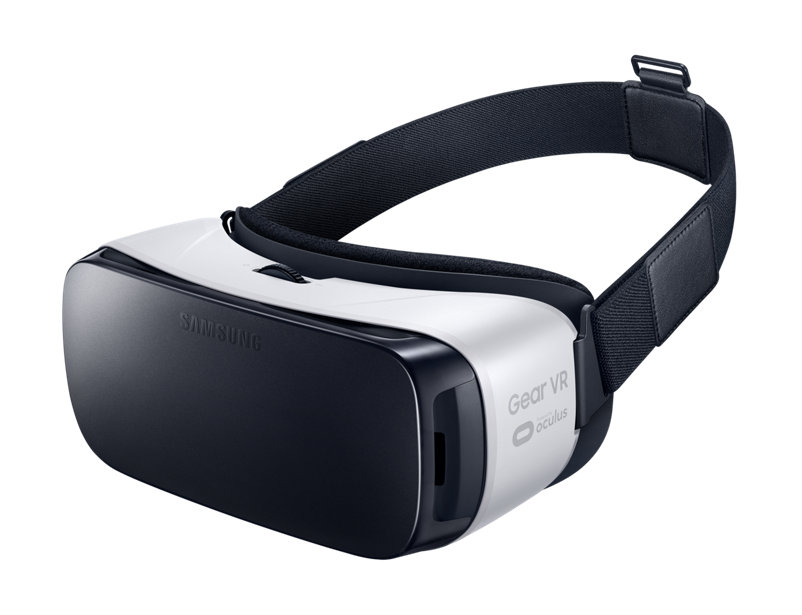
\includegraphics[scale=0.2]{../images/VR.jpeg}
  \end{columns}
\end{frame}

\section{Solution technique}
\begin{frame}
  \frametitle{Architecture}
  % \includegraphics[scale=0.2]{images/}
\end{frame}

\section{Conclusion}
\begin{frame}
  \frametitle{Conclusion}
  \begin{itemize}
  \item Faisabilité technique
  \item Impact social
  \end{itemize}
\end{frame}

\begin{frame}
  \frametitle{Questions ?}
  \begin{center}
    Question ? \\
    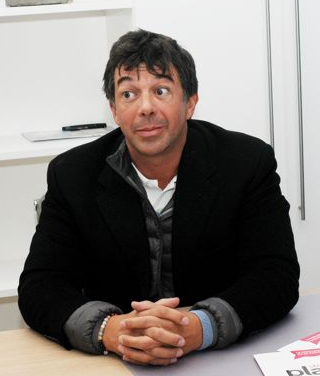
\includegraphics[scale=1.2]{../images/agent_immobilier.png}
  \end{center}
\end{frame}

\end{document}
